\documentclass[a4paper,12pt]{article}
\usepackage{graphicx}
\usepackage{geometry}
\usepackage{listings}
\usepackage{xcolor}
\usepackage{tikz}
\usetikzlibrary{arrows.meta, shapes.geometric}
\geometry{margin=1in}

\title{Practical Work 1: TCP File Transfer}
\author{}
\date{}

\begin{document}

\maketitle

\section*{Goal}
The objective of this practical is to implement a 1-to-1 file transfer system over TCP/IP using the CLI. It is based on the provided chat system and includes:
\begin{itemize}
    \item One server
    \item One client
    \item Using sockets for communication
\end{itemize}

\section*{Protocol Design}
The protocol involves the following steps:
\begin{enumerate}
    \item The server listens for incoming client connections.
    \item The client connects to the server and sends a file transfer request.
    \item Once connected, the client sends a file in chunks to the server.
    \item The server receives the file and writes it to the disk.
    \item Both the client and server close the connection after file transfer.
\end{enumerate}

\begin{figure}[h!]
    \centering
    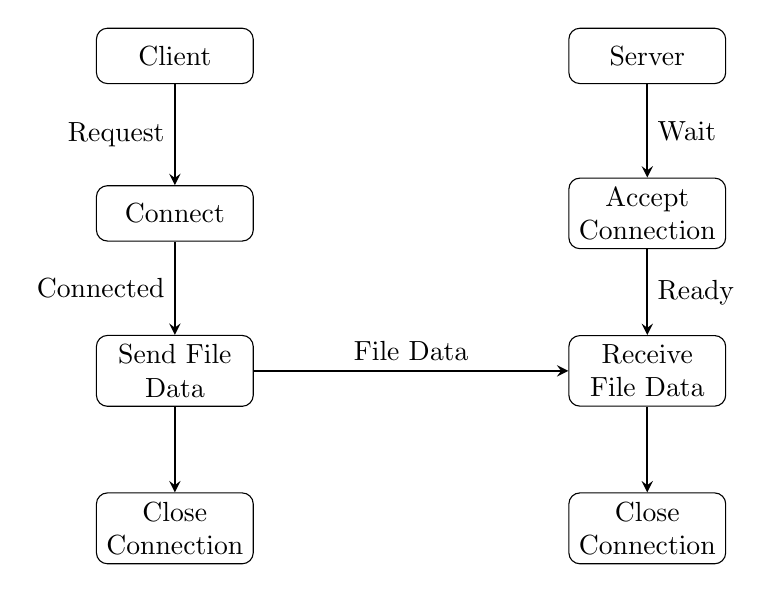
\begin{tikzpicture}[
        node distance=2cm,
        block/.style={rectangle, draw, text width=5em, text centered, rounded corners, minimum height=2em},
        arrow/.style={thick,->,>=stealth}
    ]
        % Nodes
        \node[block] (client) {Client};
        \node[block, right of=client, xshift=4cm] (server) {Server};

        % Steps
        \node[block, below of=client] (connect) {Connect};
        \node[block, below of=server] (accept) {Accept Connection};
        \node[block, below of=connect] (sendFile) {Send File Data};
        \node[block, below of=accept] (receiveFile) {Receive File Data};
        \node[block, below of=sendFile] (closeClient) {Close Connection};
        \node[block, below of=receiveFile] (closeServer) {Close Connection};

        % Arrows
        \draw[arrow] (client) -- (connect) node[midway, left] {Request};
        \draw[arrow] (server) -- (accept) node[midway, right] {Wait};
        \draw[arrow] (connect) -- (sendFile) node[midway, left] {Connected};
        \draw[arrow] (accept) -- (receiveFile) node[midway, right] {Ready};
        \draw[arrow] (sendFile) -- (receiveFile) node[midway, above] {File Data};
        \draw[arrow] (sendFile) -- (closeClient);
        \draw[arrow] (receiveFile) -- (closeServer);
    \end{tikzpicture}
    \caption{Protocol Design for TCP File Transfer}
    \label{fig:protocol-design}
\end{figure}

\section*{System Organization}
The system is organized into two main components: the client and the server. Both components utilize the socket programming API for communication.

\begin{figure}[h!]
    \centering
    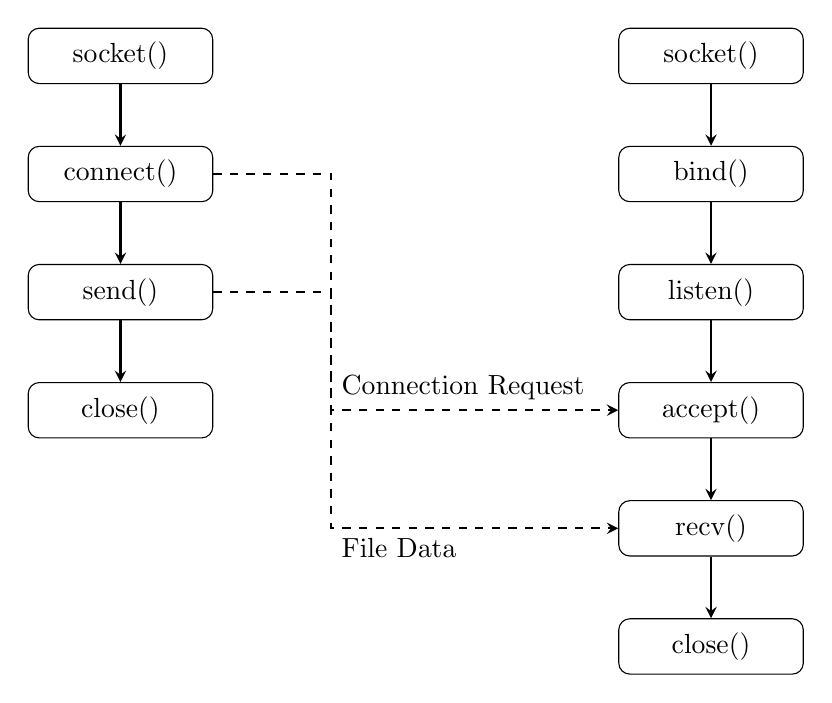
\begin{tikzpicture}[
        node distance=1.5cm,
        block/.style={rectangle, draw, text width=6em, text centered, rounded corners, minimum height=2em},
        arrow/.style={thick,->,>=stealth}
    ]
        % Client-side process
        \node[block] (clientSocket) {socket()};
        \node[block, below of=clientSocket] (clientConnect) {connect()};
        \node[block, below of=clientConnect] (clientSend) {send()};
        \node[block, below of=clientSend] (clientClose) {close()};

        % Server-side process
        \node[block, right of=clientSocket, xshift=6cm] (serverSocket) {socket()};
        \node[block, below of=serverSocket] (serverBind) {bind()};
        \node[block, below of=serverBind] (serverListen) {listen()};
        \node[block, below of=serverListen] (serverAccept) {accept()};
        \node[block, below of=serverAccept] (serverRecv) {recv()};
        \node[block, below of=serverRecv] (serverClose) {close()};

        % Arrows for Client
        \draw[arrow] (clientSocket) -- (clientConnect);
        \draw[arrow] (clientConnect) -- (clientSend);
        \draw[arrow] (clientSend) -- (clientClose);

        % Arrows for Server
        \draw[arrow] (serverSocket) -- (serverBind);
        \draw[arrow] (serverBind) -- (serverListen);
        \draw[arrow] (serverListen) -- (serverAccept);
        \draw[arrow] (serverAccept) -- (serverRecv);
        \draw[arrow] (serverRecv) -- (serverClose);

        % Connection request
        \draw[arrow, dashed] (clientConnect.east) -- ++(1.5,0) |- (serverAccept.west) node[midway, above right] {Connection Request};

        % Data transfer
        \draw[arrow, dashed] (clientSend.east) -- ++(1.5,0) |- (serverRecv.west) node[midway, below right] {File Data};

    \end{tikzpicture}
    \caption{System Organization of TCP File Transfer}
    \label{fig:system-organization}
\end{figure}

\section*{Implementation}
The implementation uses the following functions:
\begin{itemize}
    \item `socket()`: Creates a communication endpoint.
    \item `bind()`: Associates the server with an address.
    \item `listen()`: Allows the server to listen for incoming connections.
    \item `accept()`: Accepts an incoming client connection.
    \item `connect()`: Establishes a connection from the client to the server.
    \item `send()` and `recv()`: Used to send and receive file data.
\end{itemize}

\subsection*{Server Code Snippet}
Below is a simplified implementation of the server:

\begin{lstlisting}[language=Python, caption=Server Code, basicstyle=\ttfamily, keywordstyle=\color{blue}]
import socket

# Server configuration
HOST = '127.0.0.1'
PORT = 65432

# Create a socket
with socket.socket(socket.AF_INET, socket.SOCK_STREAM) as server_socket:
    server_socket.bind((HOST, PORT))
    server_socket.listen()
    print("Server listening on port", PORT)
    
    conn, addr = server_socket.accept()
    with conn:
        print("Connected by", addr)
        with open('received_file.txt', 'wb') as f:
            while True:
                data = conn.recv(1024)
                if not data:
                    break
                f.write(data)
        print("File received successfully")
\end{lstlisting}

\subsection*{Client Code Snippet}
Below is a simplified implementation of the client:

\begin{lstlisting}[language=Python, caption=Client Code, basicstyle=\ttfamily, keywordstyle=\color{blue}]
import socket

# Server configuration
HOST = '127.0.0.1'
PORT = 65432

# Create a socket
with socket.socket(socket.AF_INET, socket.SOCK_STREAM) as client_socket:
    client_socket.connect((HOST, PORT))
    print("Connected to server")
    
    # Send file
    with open('file_to_send.txt', 'rb') as f:
        while (chunk := f.read(1024)):
            client_socket.sendall(chunk)
    print("File sent successfully")
\end{lstlisting}

\section*{Responsibilities}
\begin{itemize}
    \item \textbf{Client Development:} [Duong]
    \item \textbf{Server Development:} [Duong]
    \item \textbf{Testing and Debugging:} [Duong]
    \item \textbf{Documentation:} [Duong]
\end{itemize}

\section*{Conclusion}
This practical exercise demonstrates a file transfer system over TCP/IP using a client-server model. The system was implemented using socket programming and successfully transferred files between the client and the server.

\end{document}